%===============================================================================
%===============================================================================
%
\clearpage
%
\subsection{Example-0102 \texttt{[PLAUSIBLE]}}
%
%===============================================================================
%
\subsubsection{Mathematical model}
%
We solve the following equation (both $2D$ and $3D$ domains are considered),
%
\begin{align}
    \nabla \cdot \boldsymbol{\sigma} (\boldsymbol{u}, t) = \boldsymbol{0} & &&\Omega = [0, 160] \times [0, 120] \times [0, 120], t \in [0, 5],
\end{align}
%
with time step size $\Delta_t = 1$ and $\boldsymbol{u} = [u_x,u_y]$ in $2D$ $\boldsymbol{u} = [u_x,u_y,u_z]$ in 3D. The boundary conditions in $2D$ are given by
%
\begin{align}
    u_x = u_y = 0 & &&y = 0, \\
		u_y = 8 & &&x = 160,
\end{align}
%
and in 3D by
\begin{align}
    u_x = u_z = 0 & &&x = 0, \\
    u_y = 0 & &&y = 0, \\
		u_x = 160 & &&x = 160, \\
		u_y = 8 & &&x = 160.
\end{align}
The material parameters are
\begin{align}
    E = & 10000\texttt{MPa}, \\
    \nu = & 0.3, \\
		\rho = & 5 \times 10^{-9}\texttt{tonne.mm$^3$}.
\end{align}
%
%===============================================================================
%
\subsubsection{Computational model}
%
\begin{itemize}
    \item{Commandline arguments are:}
        \subitem{float: length along x-direction}
        \subitem{float: length along y-direction}
        \subitem{float: length along z-direction (set to zero for 2D)}
        \subitem{integer: number of elements in x-direction}
        \subitem{integer: number of elements in y-direction}
        \subitem{integer: number of elements in z-direction (set to zero for 2D)}
        \subitem{integer: interpolation order (1: linear; 2: quadratic)}
        \subitem{integer: solver type (0: direct; 1: iterative)}
				\subitem{float: elastic modulus}
				\subitem{float: Poisson ratio}
				\subitem{float: displacement percentage load}
    \item{Command line arguments for tests are:}
        \subitem{160 120 0 8 6 0 1 0 10000 0.3 0.05}
				\subitem{160 120 0 16 12 0 1 0 10000 0.3 0.05}
				\subitem{160 120 0 32 24 0 1 0 10000 0.3 0.05}
				\subitem{160 120 120 8 6 6 1 0 10000 0.3 0.05}
				\subitem{160 120 120 16 12 12 1 0 10000 0.3 0.05}
				\subitem{160 120 120 32 24 24 1 0 10000 0.3 0.05}
        \subitem{160 120 0 8 6 0 2 0 10000 0.3 0.05}
				\subitem{160 120 0 16 12 0 2 0 10000 0.3 0.05}
				\subitem{160 120 0 32 24 0 2 0 10000 0.3 0.05}
				\subitem{160 120 120 8 6 6 2 0 10000 0.3 0.05}
				\subitem{160 120 120 16 12 12 2 0 10000 0.3 0.05}
				\subitem{160 120 120 32 24 24 2 0 10000 0.3 0.05}				
\end{itemize}
%
%===============================================================================
%
\subsubsection{Results}
%
\begin{figure}[h!]
    \centering 
    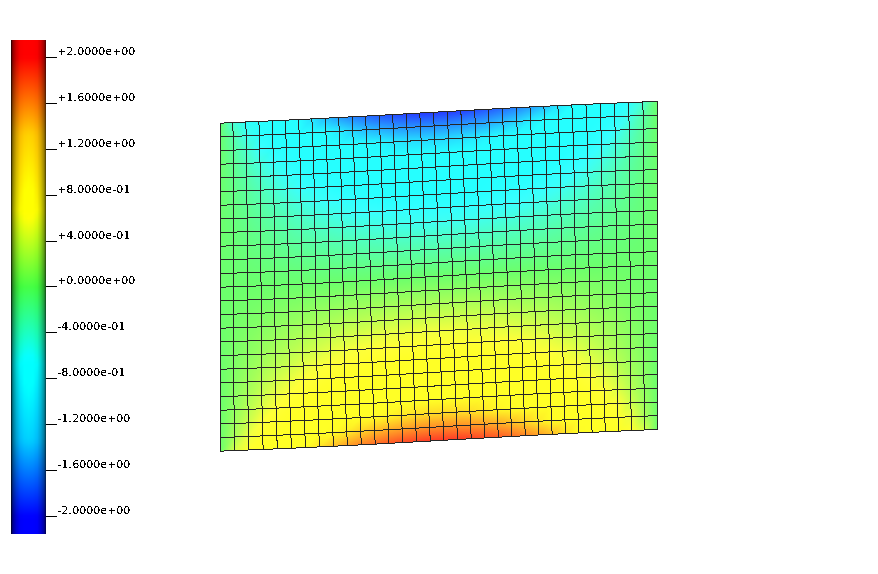
\includegraphics[width=\columnwidth]{examples/example-0102/doc/figures/l160x120x000_n32x24x00_i1_s0_shear.png} 
    \caption{Results, iron $2D$ fine mesh.}
    \label{example-0101-iron-2D-fig}
\end{figure}
%
\begin{figure}[h!]
    \centering 
    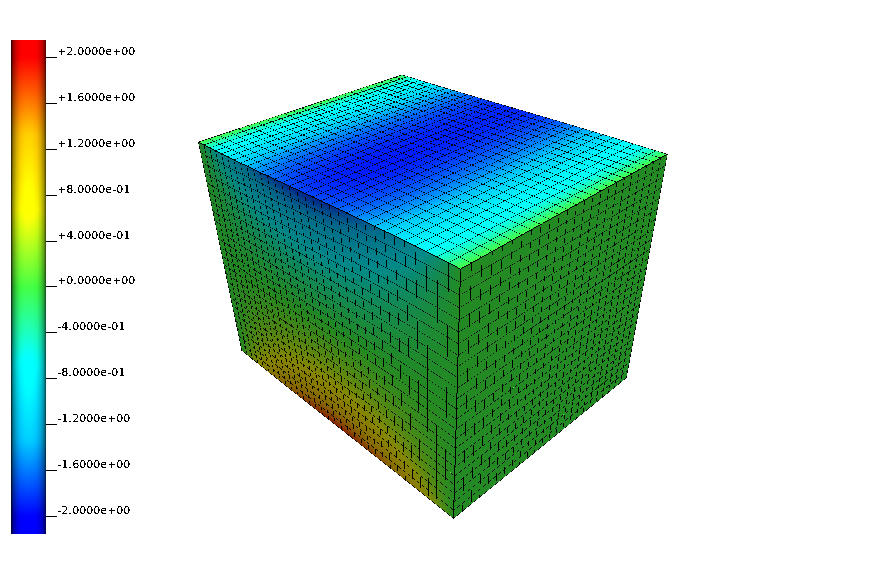
\includegraphics[width=\columnwidth]{examples/example-0102/doc/figures/l160x120x120_n32x24x24_i1_s0_shear.png} 
    \caption{Results, iron $3D$ fine mesh.}
    \label{example-0101-iron-3D-fig}
\end{figure}
%
%===============================================================================
%
\subsubsection{Validation}
%
The iron results are compared to those from Abaqus (version 2017). The figures below show selected results from the validation simulations carried out in Abaqus and provide a qualitative validation. A quantitative validation was carried out by comparing the horizontal displacement $u_x$ along the free-edge ($y=120$ for 2D and $y=z=120$ for 3D) and computing the L2-norm accodring to
\begin{align}
    L_2\texttt{-norm} = \frac{1}{N} \times \sum_{i=1}^{N} \sqrt{\left(u_{y,\texttt{abaqus}}^i-u_{y,\texttt{iron}}^i  \right)^2},
\end{align}
where $N$ is the total number of nodes along the free-edge. The results over the mesh refinements are given in Table \ref{tab:example-0101-valid-Iron-Abaqus}.
%
\begin{figure}[h!]
    \centering 
    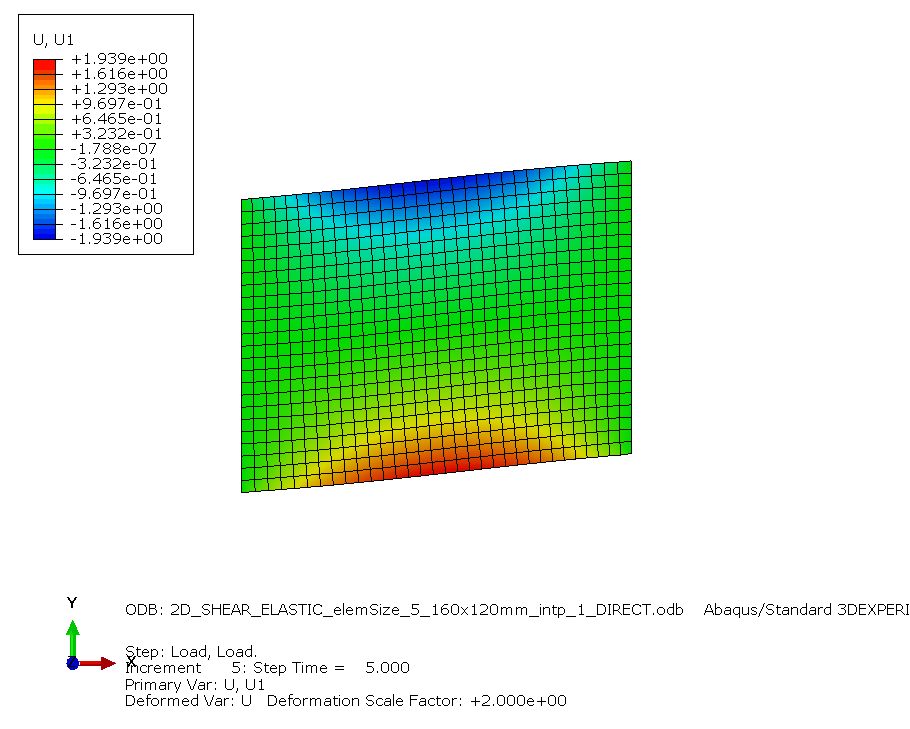
\includegraphics[width=\columnwidth]{examples/example-0102/doc/figures/2D_SHEAR_ELASTIC_elemSize_5_160x120mm_intp_1_DIRECTU1.png} 
    \caption{Results, Abaqus $2D$ fine mesh.}
    \label{example-0102-abaqus-2D-fig}
\end{figure}
%
\begin{figure}[h!]
    \centering 
    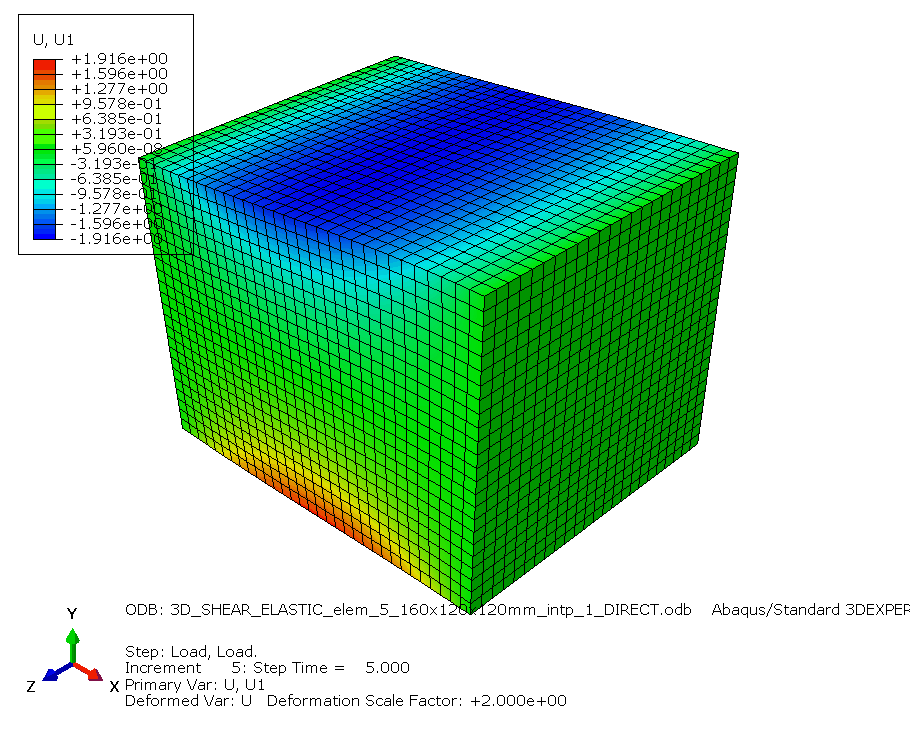
\includegraphics[width=\columnwidth]{examples/example-0102/doc/figures/3D_SHEAR_ELASTIC_elem_5_160x120x120mm_intp_1_DIRECTU1.png} 
    \caption{Results, abaqus $3D$ fine mesh.}
    \label{example-0102-abaqus-3D-fig}
\end{figure}
%
\begin{table}
	\centering
    \begin{tabular}{llll}
    Dimension & Mesh 		& $L_2\texttt{-norm}$		& Interpolation \\ \hline
    $2D$      & Coarse 	& $6.696\times 10^{-3}$	& Linear \\
    $2D$      & Medium  & $1.273\times 10^{-3}$	& Linear \\
    $2D$      & Fine  	& $2.489\times 10^{-4}$	& Linear \\
    $3D$      & Coarse  & $4.234\times 10^{-4}$	& Linear \\
    $3D$      & Medium  & $4.184\times 10^{-5}$	& Linear \\
		$3D$			&	Fine 		&	$3.781\times 10^{-6}$	& Linear \\
    $2D$      & Coarse 	& $3.036\times 10^{-4}$	& Quadratic \\
    $2D$      & Medium  & $6.099\times 10^{-5}$	& Quadratic \\
    $2D$      & Fine  	& $1.089\times 10^{-5}$	& Quadratic \\
    $3D$      & Coarse  & \ldots 									& Quadratic \\
    $3D$      & Medium  & \ldots									& Quadratic \\
		$3D$			&	Fine 		&	\ldots									& Quadratic \\				
    \end{tabular}
		\caption{Quantiative error between Abaqus 2017 and iron simulations for linear elastic shear}
		\label{tab:example-0102-valid-Iron-Abaqus}
\end{table}
%===============================================================================
%===============================================================================
